\setlength{\parskip}{\baselineskip}


\chapter{Introducción}
\label{cap:introduccion}


\section{Contexto}

Las redes Peer-to-Peer (P2P) representan un modelo de comunicación descentralizado en el que todos los nodos participan de forma equitativa, actuando tanto como clientes como servidores. Este paradigma, alternativo al modelo cliente-servidor tradicional, ha transformado la forma en que compartimos información y utilizamos los recursos en línea. Su impacto ha sido especialmente notable en el ámbito del intercambio de archivos, donde su capacidad para distribuir grandes volúmenes de datos sin depender de servidores centralizados ha supuesto una revolución tecnológica \cite{schollmeier2001}.


\begin{figure}[h]
    \centering
    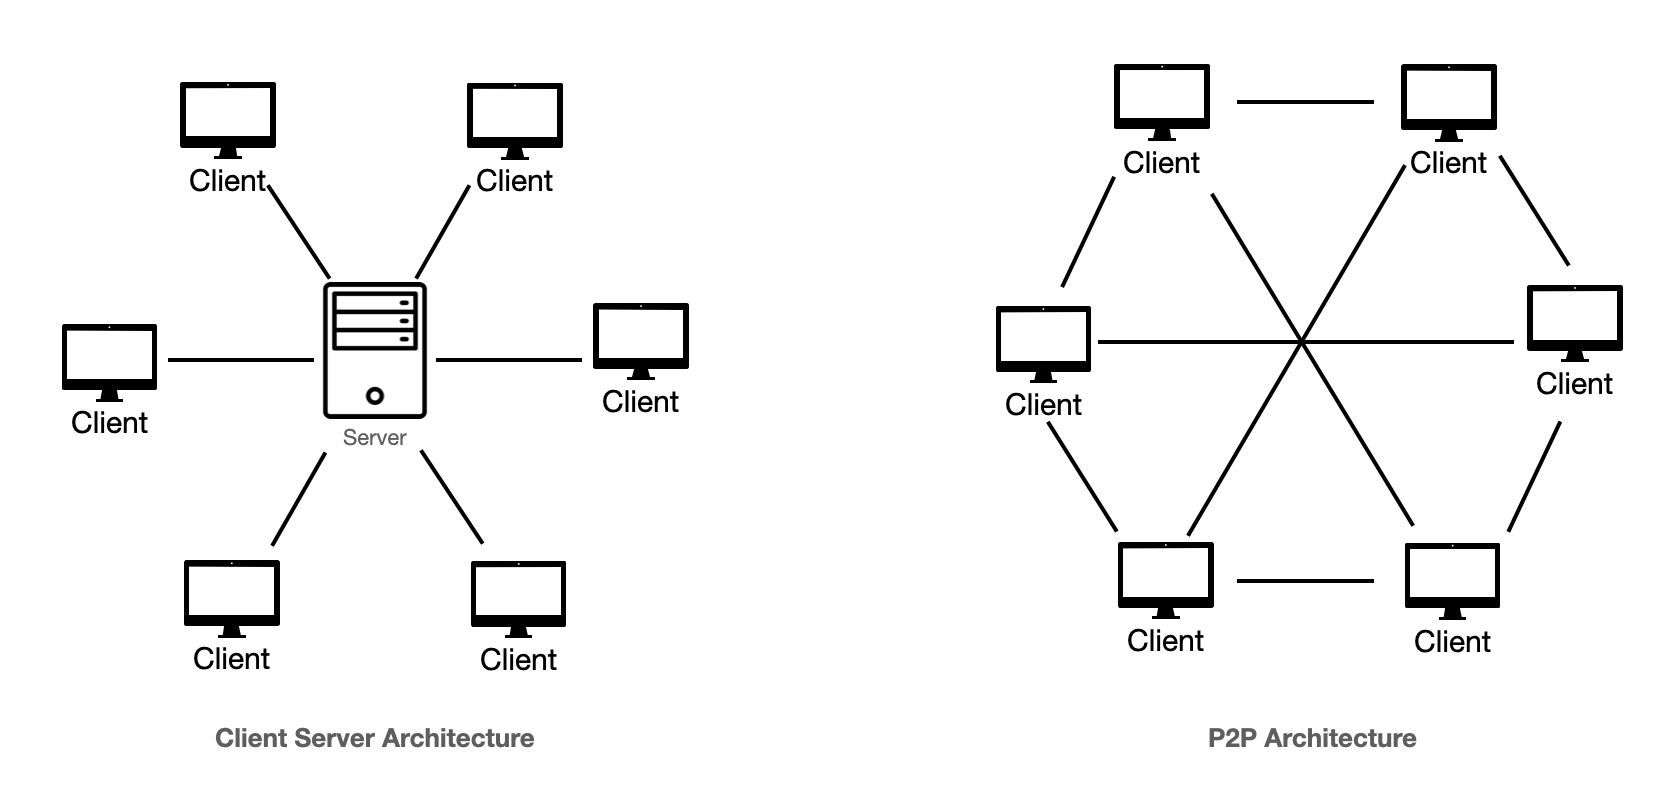
\includegraphics[width = 0.5\textwidth]{Imagenes/Vectorial/client-server-vs-p2p}
    \caption{Comparaci\'on entre arquitectura cliente-servidor y arquitectura P2P}
    \label{fig:clientVsp2p}
\end{figure}


El inicio de las redes P2P modernas se remonta a finales de la década de 1990, con la aparición de Napster en 1999. Napster introdujo un modelo centralizado en el que los usuarios podían buscar y descargar archivos, principalmente música, a través de un servidor que indexaba todos los contenidos disponibles. Esta plataforma, aunque técnicamente no era completamente P2P debido a su dependencia de un servidor central, fue pionera en popularizar el intercambio de archivos entre pares.


Sin embargo, Napster enfrentó múltiples desafíos legales, principalmente por el intercambio no autorizado de material protegido por derechos de autor. Estos problemas llevaron a su cierre en 2001, pero también impulsaron el desarrollo de alternativas más descentralizadas que no dependían de un punto único de control.


La caída de Napster marcó el comienzo de una segunda generación de redes P2P, más resilientes y descentralizadas. Plataformas como Gnutella y eDonkey surgieron como respuesta a la vulnerabilidad inherente de los sistemas centralizados. Gnutella, por ejemplo, permitió que cada nodo en la red actuara de forma completamente independiente, eliminando la necesidad de un servidor central.


Estas redes introdujeron nuevos retos técnicos, como la búsqueda eficiente de archivos en una red distribuida y el manejo de grandes volúmenes de tráfico. Para abordar estos problemas, se desarrollaron algoritmos más avanzados para la localización de recursos y técnicas de segmentación de archivos para optimizar la transferencia de datos.


La llegada de BitTorrent en 2001 marcó un nuevo hito en la evolución de las redes P2P. Este protocolo introdujo un enfoque innovador para el intercambio de archivos al dividirlos en fragmentos más pequeños. Los usuarios podían descargar estos fragmentos desde múltiples fuentes simultáneamente, lo que mejoraba significativamente la velocidad y la eficiencia de las transferencias. Además, BitTorrent redujo la carga sobre los nodos individuales al permitir que los usuarios que habían descargado partes de un archivo las compartieran inmediatamente con otros \cite{cohen2003}.


A lo largo de los años, las redes P2P han evolucionado para abarcar aplicaciones más allá del intercambio de archivos. En la actualidad, estas tecnologías son fundamentales en áreas como el streaming de vídeo, los juegos en línea y, más recientemente, las plataformas basadas en blockchain como Bitcoin. Este último caso destaca por su capacidad para descentralizar no solo la transferencia de datos, sino también el control financiero, mediante un registro distribuido y seguro.



\section{Motivación}
Introducción al tema del TFM.


\section{Objetivos}
Descripción de los objetivos del trabajo.


\section{Plan de trabajo}
Aquí se describe el plan de trabajo a seguir para la consecución de los objetivos descritos en el apartado anterior.


\section{Explicaciones adicionales sobre el uso de esta plantilla}
Si quieres cambiar el \textbf{estilo del título} de los capítulos, edita \verb|TeXiS\TeXiS_pream.tex| y comenta la línea \verb|\usepackage[Lenny]{fncychap}| para dejar el estilo básico de \LaTeX.

Si no te gusta que no haya \textbf{espacios entre párrafos} y quieres dejar un pequeño espacio en blanco, no metas saltos de línea (\verb|\\|) al final de los párrafos. En su lugar, busca el comando  \verb|\setlength{\parskip}{0.2ex}| en \verb|TeXiS\TeXiS_pream.tex| y aumenta el valor de $0.2ex$ a, por ejemplo, $1ex$.

TFMTeXiS se ha elaborado a partir de la plantilla de TeXiS\footnote{\url{http://gaia.fdi.ucm.es/research/texis/}}, creada por Marco Antonio y Pedro Pablo Gómez Martín para escribir su tesis doctoral. Para explicaciones más extensas y detalladas sobre cómo usar esta plantilla, recomendamos la lectura del documento \texttt{TeXiS-Manual-1.0.pdf} que acompaña a esta plantilla.

El siguiente texto se genera con el comando \verb|\lipsum[2-20]| que viene a continuación en el fichero .tex. El único propósito es mostrar el aspecto de las páginas usando esta plantilla. Quita este comando y, si quieres, comenta o elimina el paquete \textit{lipsum} al final de \verb|TeXiS\TeXiS_pream.tex|

\subsection{Texto de prueba}


\lipsum[2-20]